% This is based on the LLNCS.DEM the demonstration file of
% the LaTeX macro package from Springer-Verlag
% for Lecture Notes in Computer Science,
% version 2.4 for LaTeX2e as of 16. April 2010
%
% See http://www.springer.com/computer/lncs/lncs+authors?SGWID=0-40209-0-0-0
% for the full guidelines.
%
\documentclass{llncs}

\usepackage{graphicx}
\usepackage{verbatim}
\usepackage{fancyhdr}
\usepackage{listings}
\usepackage{color}
\usepackage{booktabs}

\definecolor{dkgreen}{rgb}{0,0.6,0}
\definecolor{gray}{rgb}{0.5,0.5,0.5}
\definecolor{mauve}{rgb}{0.58,0,0.82}

\lstset{frame=tb,
  language=Prolog,
  aboveskip=3mm,
  belowskip=3mm,
  showstringspaces=false,
  columns=flexible,
  basicstyle={\small\ttfamily},
  numbers=none,
  numberstyle=\tiny\color{gray},
  keywordstyle=\color{blue},
  commentstyle=\color{dkgreen},
  stringstyle=\color{mauve},
  breaklines=true,
  breakatwhitespace=true,
  tabsize=3
  }

\begin{document}

\title{Skyscraper\\Decision Problem solved with Constraint Logic Programming}
%
\titlerunning{Skyscraper}  % abbreviated title (for running head)
%                                     also used for the TOC unless
%                                     \toctitle is used
%
\author{André Cruz\inst{1} \and Edgar Carneiro\inst{2}}
%
\authorrunning{André Cruz \and Edgar Carneiro} % abbreviated author list (for running head)
%
%%%% list of authors for the TOC (use if author list has to be modified)
\tocauthor{André Cruz and Edgar Carneiro}
%
\institute{Faculdade de Engenharia da Universidade do Porto\\ Rua Roberto Frias, sn, 4200-465 Porto, Portugal,\\
\texttt{FEUP-PLOG, Class 3MIEIC01, Group Skyscraper\_5}}

\maketitle              % typeset the title of the contribution

\begin{abstract}
This article presents a Constraint Logic Programming approach to define and ultimately solve the puzzle ``Skyscraper''.
The purposed solution is independent of board size and number of restrictions.
The solver can also be presented with a partially-filled board, as is customary in larger boards.
We also dynamically generate ``Skyscraper'' puzzles, of different sizes and with varying difficulty.
Results show that ``Skyscraper'' is a prime example for being solved with CLP, as the solution's code is brief, efficient, and simple to understand.

\keywords{Skyscraper, Constraint Logic Programming, Sicstus, PLOG, FEUP}
\end{abstract}
%
\section{Introduction}
%
The ``Skyscraper'' puzzles consists of an NxN grid with some clues along its sides. This type of puzzles combines the row and column constraints of Sudoku with external clue values that re-imagine each row or column of numbers as a road full of skyscrapers of varying height.

We model the presented puzzle as a Constraint Satisfaction Problem (CSP), therefore representing it by a set of domain variables, their domains, and a set of restrictions.

Constraint Logic Programming (CLP) is a merger of two declarative paradigms: constraint solving and logic programming. Viewing the subject rather broadly, constraint logic programming can be said to involve the incorporation of constraints and constraint “solving” methods in a logic-based language. We refer the reader to \cite{jaffar_maher_1994} for more on this subject.

In this paper, section 2 begins by describing the problem at hand in detail. Section 3 presents our approach to solving this decision problem using Prolog, as well as the finer grained details of the CSP modelling. The choice of labeling strategy is also explained. Section 4 describes the presentation of the solution in a user-friendly manner. Section 5 presents our results performance-wise, as well as a set of key issues we discovered while developing the code. Finally, section 6 presents the conclusion and future work.

%
\section{Problem Description}
%
The ``Skyscraper'' puzzle consists of an NxN grid with some clues along its sides. The objective is to place a skyscraper (represented by its height) in each square, with a height between 1 and N, so that each row and column contains each digit exactly once. In addition, the number of visible skyscrapers, as viewed from the direction of each clue, is equal to the value of the clue. Note that higher skyscrapers block the view of lower skyscrapers located behind them. A comprehensive booklet with the puzzle's rules can be found here \cite{skyscrapers_booklet}.

The difficulty of the puzzle can vary according to three factors: the size of the board, the number of restrictions along the side of the board, and the possible hints in the board itself (it is common to present larger boards partially filled).

\begin{figure}[h!]
\begin{center}
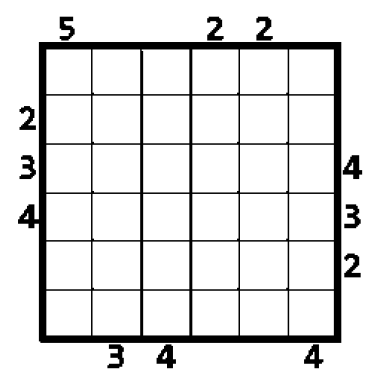
\includegraphics[height=4.5cm,width=4.5cm]{images/skyscraper_unsolved.png}
\caption{Unsolved 6x6 Skyscraper puzzle}
\label{Figure 1}
\end{center}
\end{figure}

\begin{figure}[h!]
\begin{center}
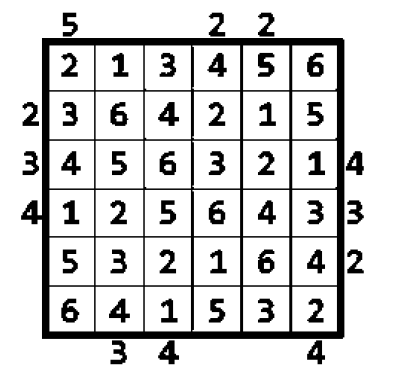
\includegraphics[height=4.5cm,width=4.5cm]{images/skyscraper_solved.png}
\caption{Solved 6x6 Skyscraper puzzle}
\label{Figure 2}
\end{center}
\end{figure}

%
\section{Approach}
We present a Constraint Logic Programming approach to define and ultimately solve the puzzle ``Skyscraper''. In order to accomplish this, we use the clp(fd) --- Constraint Logic Programming over Finite Domains --- library in sicstus Prolog. For more information on this prolog implementation, and said library, we refer the reader to \cite{sterling_shapiro_warren_2010} and \cite{carlsson_fruhwirth_2016}.

Regarding the implementation of Skyscraper in Prolog, we decided to represent the board's matrix as a list of lists, whose elementary units are integer numbers, representing the height of the skyscraper in that position.
Elements whose value is not known are represented by  a `\_', therefore representing in Prolog non-instantiated values.

For the restrictions along the side of the grid, we use a list of lists, the first of which being the top restrictions, and the rest following in counter-clockwise order. If the restriction for a certain row or column is undefined, a `0' is used in its position.

\begin{figure}[h!]
\begin{center}
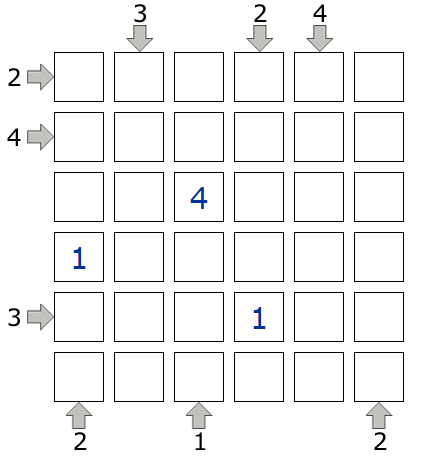
\includegraphics[height=5cm,width=5cm]{images/example_skyscraper.png}
\caption{Example of a skyscraper puzzle followed by its representation in PROLOG}
\label{Figure 3}
\end{center}
\end{figure}
\noindent\begin{minipage}{.48\textwidth}
\begin{lstlisting}[frame=tlrb, caption=Prolog grid representation]
testBoard([
  [_, _, _, _, _, _],
  [_, _, _, _, _, _],
  [_, _, 4, _, _, _],
  [1, _, _, _, _, _],
  [_, _, _, 1, _, _],
  [_, _, _, _, _, _]
]).
\end{lstlisting}
\end{minipage}\hfill
\begin{minipage}{.42\textwidth}
\begin{lstlisting}[frame=tblr, caption=Prolog representation of border restrictions]
testRestrictions([
  [0, 3, 0, 2, 4, 0],
  [2, 4, 0, 0, 3, 0],
  [2, 0, 1, 0, 0, 2],
  [0, 0, 0, 0, 0, 0]
]).
\end{lstlisting}
\end{minipage}\hfill

%
\subsection{Decision Variables}

The decision variables associated with a skyscraper puzzle are: the numbers of the board's grid, and the numbers of the restrictions along the side of the grid.
The domain of the elements of the grid, according to the puzzle's rules \cite{skyscrapers_booklet}, is between 1 and N.
The domain of the restrictions along the side is also between 1 and N. Because this restrictions can be defined, we extended this domain to include the value 0, as this value internally represents an undefined restriction.

The application of domain restrictions is done in the following code.

\noindent\begin{minipage}{.44\textwidth}
\begin{lstlisting}[frame= tblr, caption=Row domain restrictions]
restrictBoardDomain([], _).
restrictBoardDomain([Row | Board], N) :-
  length(Row, N),
  domain(Row, 1, N),
  all_distinct(Row),
  restrictBoardDomain(Board, N).
\end{lstlisting}
\end{minipage}\hfill
\begin{minipage}{.5\textwidth}
\begin{lstlisting}[frame=tblr, caption=Column all elements distinct]
all_distinct_columns(_, 0) :- !.
all_distinct_columns(Board, N) :-
  N > 0, !,
  getBoardCol(Board, N, Col),
  all_distinct(Col),
  NewN is N - 1,
  all_distinct_columns(Board, NewN).
\end{lstlisting}
\end{minipage}\hfill
\begin{lstlisting}[frame=tblr, caption=Constraints for the Border restrictions domains]
sidesDomain(Size, [List | Rest]) :-
  length(List, Size),
  domain(List, 0, Size),
  sidesDomain(Size, Rest).
sidesDomain(_, []).
\end{lstlisting}

%
\subsection{Constraints}

The restrictions defined for the puzzle in Prolog are fairly faithful to the ones from the rules. The uniqueness of variables along their columns and rows is fairly straightforward to implement using the \textit{all\_distinct} predicate (see the listings 1.3 and 1.4 in section \textbf{Decision Variables}). Therefore, the challenge involving the project was the addition of PROLOG restrictions to implement the missing rule: assuring that the number outside the grid would indeed control the number of `visible buildings'.\\

The solution we came up to implement that last rule was a \textit{logic XOR}, \textbf{\#\textbackslash}: the element being analyzed was either the maximum so far, and the following buildings with smaller height wouldn't count towards the side restriction; or it was not a maximum building, therefore not visible along the side, and the count of visible buildings would stay the same.

When the row/column being analyzed had no more elements, the number of visible buildings (a domain variable in itself) would be equal, \#=, to the corresponding side restraining value. The predicate would be called for each line/ column for each of the four possible directions: left to right, right to left, top to bottom and bottom to top.

\begin{lstlisting}[frame=tblr, caption=Constraint that assures correct number of visible buildings ]	
/**
 * Apply restrictions to Row.
 * +Predicate Order in which elements are analyzed - fetches an element.
 * +Num is the number of visible skyscrapers according to the above order.
 */
applyToRow(Num, Row, Max, GetElement) :-
  call(GetElement, Row, El, RemainderRow),
  NewNum #>= 0,
  (El #> Max #/\ NewMax #= El #/\ NewNum #= Num - 1) #\/
  (El #=< Max #/\ NewMax #= Max #/\ NewNum #= Num),
  applyToRow(NewNum, RemainderRow, NewMax, GetElement).
applyToRow(0, [], _, _).
\end{lstlisting}

%
\subsection{Search Strategy}

The labeling strategy implemented in the program was the \textbf{\textit{ffc}}, also known as \textit{most\_constrained}. This labeling strategy makes use of the most constrained heuristic: ` a variable with the smallest domain is selected, breaking ties by (a) selecting the variable that has the most constraints suspended on it and (b) selecting the leftmost one'\cite{carlsson_fruhwirth_2016}.  We opted for this heuristic as it would be the one providing faster and more efficient solutions for the skyscraper puzzle. Naturally the default values were not appropriate for this representation, as the order in which the variables were presented had no intrinsic value (labeling left-to-right was not particularly useful). Having in mind the kind of constraints used in the modeling of the problem, a certain value was more likely to stick (to not backtrack) if its variable had a tighter domain; and, if it did backtrack, it would do so less often.

%
\section{Solution Presentation}

For the solution presentation in text mode the predicate \textit{printBoard} is used. If run as \textbf{\textit{printBoard(+Board)}}, it only prints the given board in a user friendly way. However, if run as \textbf{\textit{printBoard(+Board, +Restrictions)}} it will print the board in a user friendly way while also displaying the boarder restrictions being applied to each row or column. The predicate makes use of helper predicates such as \textbf{\textit{printRow(+Row)}}, that prints the given row and \textbf{\textit{printHBorder(+Length)}}, that prints the horizontal border at the top and the bottom. All this predicates are defined in the file \textbf{\textit{display.pl}}.

\begin{figure}[h!]
\begin{center}
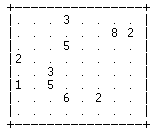
\includegraphics[height=3cm,width=3cm]{images/printBoard1.png}
\caption{Example of a call to printBoard/1}
\label{Figure 3}
\end{center}
\end{figure}

\begin{figure}[h!]
\begin{center}
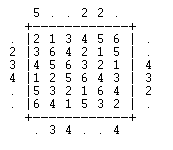
\includegraphics[height=4cm,width=4cm]{images/printBoard21.png}
\caption{Example of a call to printBoard/2 with a solved board}
\label{Figure 4}
\end{center}
\end{figure}

%
\section{Results}

The group tried to make extensive and exhaustive tests to be able to extract comprehensive conclusions regarding the obtained results.

The results of several tests that the group made were:

\begin{table}[]
\centering
\caption{Each of the values is the result of the average of several tests made}
\label{Results Tablel}
\begin{tabular}{@{}ccc@{}}
\toprule
\multicolumn{1}{c|}{\textbf{Board Size}} & \multicolumn{1}{c|}{\textbf{Time /s}} & \textbf{Backtracks} \\ \midrule
4x4                                      & 0.0                                 & 9                   \\ \midrule
5x5                                      & 0.047                                 & 659                 \\ \midrule
6x6                                      & 0.291                                 & 5438                \\ \midrule
7x7                                      & 10.489                                & 159196              \\ \midrule
8x8                                      & 18.239                                & 315893              \\ \bottomrule
\end{tabular}
\end{table}

In the end, the conclusions the group came up with were:
\begin{itemize}
	\item There is an exponential relation between the board size and time taken to solve the puzzle. For smaller boards the difference in board size affects slightly the difference of times (board size 4 to board size 5, differences of around 0.05s). However in bigger boards the difference of board sizes affect time fiercely (board size 6 to board size 7, differences of around 10s).\\

\begin{figure}[h!]
\begin{center}
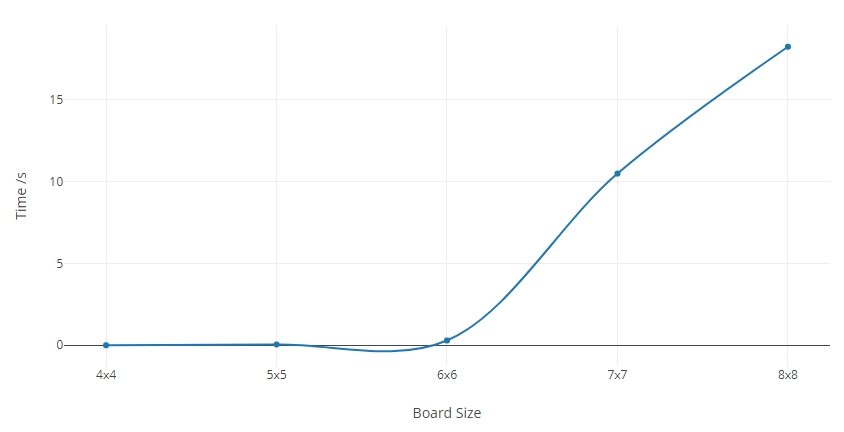
\includegraphics[height=6cm,width=12cm]{images/graph1.png}
\caption{Relation between board size and time taken to find a solution.}
\label{Figure 5}
\end{center}
\end{figure}

	\item There is a strong correlation between the number of backtracks (and the other statistics, such as \textit{Resumptions, Entailments, Prunings and Constraints created}) and time. The higher the value of the statistics the higher the time it took the program to solve the puzzle.\\

\begin{figure}[h!]
\begin{center}
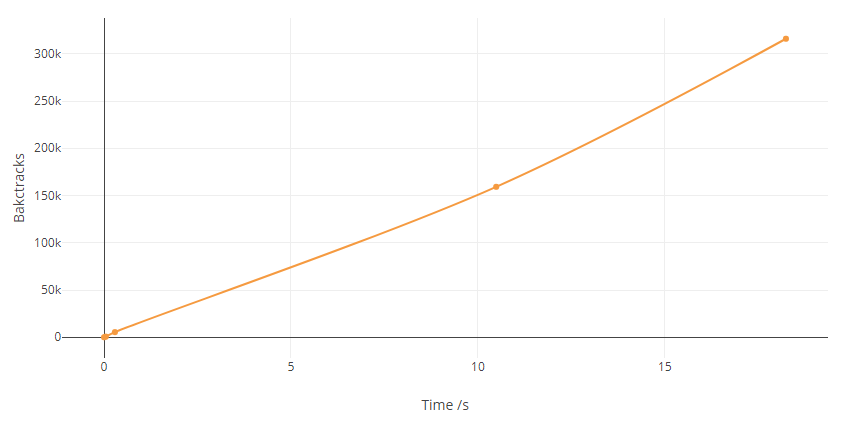
\includegraphics[height=6cm,width=12cm]{images/graph2.png}
\caption{Relation between number of backtracks and time to solve the puzzle}
\label{Figure 6}
\end{center}
\end{figure}
	
	\item It is also worth noticing that, for the same board size, a puzzle with a higher number of side restrictions is faster to solve. This was expected, as the board's domain variables have stricter constraints, leading to a decreased number of backtracks.
\end{itemize}

%
\section{Conclusion and Future Work}

We believe that our knowledge about Logic Programming was deeply increased, with everything we had proposed to do being accomplished in the required time.

The program developed has no limitations regarding board size or problem generation, despite becoming evidently slower with larger board sizes. Therefore, the only way possible to improve the developed application would be by improving the solver's efficiency. However, the group tried fiercely to make that improve by trying out several approaches, but in the end the best solution was the one presented here.

It is also evident that Constraint Logic Programming revealed itself to be an extremely powerful tool, extremely appropriate to tackle problems like the one presented, resulting in a faithful and straightforward representation of the problem, and much faster development.

To sum up, despite Constraint Logic Programming being a unique programming paradigm, rather distinct from classical ones, we quickly got used to it and learnt to appreciate the cons and pros that it presents, thus having it culminate in a project we are proud to present.

%
\section{Acknowledgements}
This article was written for the course unit ``Logic Programming'', from the Master in Informatics and Computing Engineering, a course in the Faculty of Engineering of the University of Porto.


%
% ---- Bibliography ----
%
\clearpage
\addcontentsline{toc}{section}{References}
\renewcommand\refname{References}
\bibliography{myrefs}
\bibliographystyle{ieeetr}


\newpage
\appendix
\section{Appendix}

\huge\textbf{skyscraper.pl}
\begin{lstlisting}[language=Prolog]
:- include('solver.pl').
:- include('display.pl').
:- include('test_data.pl').
:- include('generator.pl').

%Predicate to run the default puzzle
skyscraper :-
  nl, write('Skyscraper!'), nl, nl,
  testRestrictions(R),
  R = [Up | _Rest],
  length(Up, Size),
  solveBoard(Size, B, R),
  printBoard(B, R).
\end{lstlisting}
\newpage

\huge\textbf{solver.pl}
\begin{lstlisting}[language=Prolog]
:- use_module(library(clpfd)).
:- use_module(library(lists)).

/**
 * Domain restriction
 */
sidesDomain(Size, [List | Rest]) :-
  length(List, Size),
  domain(List, 0, Size),
  sidesDomain(Size, Rest).
sidesDomain(_, []).

restrictBoardDomain([], _).
restrictBoardDomain([Row | Board], N) :-
  length(Row, N),
  domain(Row, 1, N),
  all_distinct(Row),
  restrictBoardDomain(Board, N).

all_distinct_columns(_, 0) :- !.
all_distinct_columns(Board, N) :-
  N > 0, !,
  getBoardCol(Board, N, Col),
  all_distinct(Col),
  NewN is N - 1,
  all_distinct_columns(Board, NewN).


% Get the nth1 column of the given Board (1 indexed)
getBoardCol([], _, []).
getBoardCol([Row | Board], N, [El | Col]) :-
  element(N, Row, El),
  getBoardCol(Board, N, Col).


%% Gets the FIRST element of a given row
getFirstElement([Element | RemainderRow], Element, RemainderRow).

%% Gets the LAST element of a given row
getLastElement(Row, Element, RemainderRow) :-
  append(RemainderRow, [Element], Row).


%% LEFT to RIGHT
applyLeftToRight(Num, Row) :-
  applyToRow(Num, Row, 0, getFirstElement).

%% RIGHT to LEFT
applyRightToLeft(Num, Row) :-
  applyToRow(Num, Row, 0, getLastElement).

/**
 * Apply restrictions to Row.
 * +Predicate Order in which elements are analyzed - fetches an element.
 * +Num is the number of visible skyscrapers according to the above order.
 */
applyToRow(Num, Row, Max, GetElement) :-
  call(GetElement, Row, El, RemainderRow),
  NewNum #>= 0,
  (El #> Max #/\ NewMax #= El #/\ NewNum #= Num - 1) #\
  (El #=< Max #/\ NewMax #= Max #/\ NewNum #= Num),
  applyToRow(NewNum, RemainderRow, NewMax, GetElement).
applyToRow(0, [], _, _).

/**
 * Applies restrictions Horizontally along the board
 * +Predicate is the predicate used to apply restrictions on the fetched Row.
 */
applyAllHorizontalRestrictions([0 | Rest], [_ | Rows], Predicate) :-
  applyAllHorizontalRestrictions(Rest, Rows, Predicate).
applyAllHorizontalRestrictions([N | Rest], [Row1 | Rows], Predicate) :-
  call(Predicate, N, Row1),
  applyAllHorizontalRestrictions(Rest, Rows, Predicate).
applyAllHorizontalRestrictions([], [], _).

/**
 * Applies restrictions Vertically along the board
 * +Predicate is the predicate used to apply restrictions on the fetched Column.
 */
applyAllVerticalRestrictions(Restrictions, Board, Predicate) :-
  applyAllVerticalRestrictions(Restrictions, Board, Predicate, 1).
applyAllVerticalRestrictions([0 | Rest], Board, Predicate, Count) :-
  NewCount is Count + 1,
  applyAllVerticalRestrictions(Rest, Board, Predicate, NewCount).
applyAllVerticalRestrictions([N | Rest], Board, Predicate, Count) :-
  NewCount is Count + 1,
  getBoardCol(Board, Count, Col),
  call(Predicate, N, Col),
  applyAllVerticalRestrictions(Rest, Board, Predicate, NewCount).
applyAllVerticalRestrictions([], _, _, _).


/**
 *  +Sides -> a list of lists, each of which represents the restrictions on the side of the board (number of visible buildings).
 *      -> in order: [TopRestrictions, LeftRestrictions, BottomRestrictions, RightRestrictions]
 *      -> elements of list are in range [0,N], 0 meaning an undefined restriction
 *      -> elements correspond to restrictions in top->bottom (left/right lists) or left->right (top/bottom lists) order
 *  -Board -> a list of lists (a matrix)
 */
solveBoard(Size, Board, Sides) :-
  Sides = [Top, Left, Bottom, Right],
  sidesDomain(Size, Sides),

  % Domain
  length(Board, Size),
  restrictBoardDomain(Board, Size),
  all_distinct_columns(Board, Size),

  % Apply restrictions to board rows/columns
  applyAllHorizontalRestrictions(Left, Board, applyLeftToRight),
  applyAllHorizontalRestrictions(Right, Board, applyRightToLeft),
  applyAllVerticalRestrictions(Top, Board, applyLeftToRight),
  applyAllVerticalRestrictions(Bottom, Board, applyRightToLeft),

  append(Board, FlatBoard),
  append(Sides, FlatSides),
  append(FlatBoard, FlatSides, DomainVariables),
  labeling([ffc], DomainVariables).

\end{lstlisting}
\newpage

\huge\textbf{generator.pl}
\begin{lstlisting}[language=Prolog]
:- use_module(library(lists)).
:- use_module(library(random)).
:- include('solver.pl').

% Restrict the number of constraints shown , according to the probability
restrictVarsInSides([], _).
restrictVarsInSides([First | Rest], Probability) :-
  restrictVarsInRow(First, Probability),
  restrictVarsInSides(Rest, Probability).

% Restrict the number of constraints shown , according to the probability
restrictVarsInRow([], _).
restrictVarsInRow([V1 | Vars], Probability) :-
  maybe(Probability), !,
  V1 #\= 0,
  restrictVarsInRow(Vars, Probability).
restrictVarsInRow([_ | Vars], Probability) :-
  restrictVarsInRow(Vars, Probability).

/**
 * Generates boards of differente difficulty according the given probability.
 * +The probability will control the amount of Restrictions that are shown.
 */
generateBoardEasy(Size, Board, Sides) :-
  generateBoard(Size, Board, Sides, 0.95).
generateBoardMedium(Size, Board, Sides) :-
  generateBoard(Size, Board, Sides, 0.8).
generateBoardHard(Size, Board, Sides) :-
  generateBoard(Size, Board, Sides, 0.65).
generateBoard(Size, Board, Sides, Probability) :-
  setrand(100),
  length(Sides, 4),
  sidesDomain(Size, Sides),
  restrictVarsInSides(Sides, Probability),

  solveBoard(Size, Board, Sides).

/*
generateBoardUniqueSol(Size, Board, Sides) :-
  setrand(200),
  length(Sides, 4),
  sidesDomain(Size, Sides),
  Probability = 1,
  restrictVarsInSides(Sides, Probability),
  findall(B, solveBoard(Size, B, Sides), [Board]).
*/ % badbadnotgood backtracking

% Size = 8, generateBoardEasy(Size, B, S), printBoard(B, S), solveBoard(Size, SB, S), printBoard(SB, S).
% Size = 8, generateRandomBoard(Size, Board, Sides), printBoard(Board, Sides), solveBoard(Size, SameBoard, Sides), printBoard(SameBoard, Sides), Board = SameBoard.
% Size = 6, generateRandomBoard(Size, Board, Sides), printBoard(Board, Sides), solveBoard(Size, SameBoard, Sides), Board = SameBoard.

\end{lstlisting}
\newpage

\huge\textbf{display.pl}
\begin{lstlisting}[language=Prolog]
%Dictionary for user friendly visualization of elements
translate(0, '.').
translate(P, P).

% printBoard(+Board)
%% prints the given board on the screen
printBoard(Board) :-
  Board = [Row | _],
  length(Row, RowLength),
  printHBorder(RowLength),
  printBoardAux(Board),
  printHBorder(RowLength).

printBoardAux([]) :- !.
printBoardAux([Row | Board]) :-  
  printRow(Row), nl,
  printBoardAux(Board).

% printBoard(+Board, +Restrictions)
%% prints the given board, and all the provided side restrictions
printBoard(Board, Restrictions) :- !,
  Restrictions = [Top, Left, Bottom, Right],
  write('   '), printRowAux(Top), nl,
  length(Top, RowLength), 
  write('  '), printHBorder(RowLength),
  printBoard(Board, Left, Right),
  write('  '), printHBorder(RowLength),
  write('   '), printRowAux(Bottom), nl, nl.

% printBoard(+Board, +LeftRestrictions, +RightRestrictions)
%% prints the given board, and the provided side restrictions for left and right
printBoard([], [], []) :- !.
printBoard([Row | Board], [L1 | Left], [R1 | Right]) :-
  translate(L1, SymbL), translate(R1, SymbR),
  write(SymbL), write(' '),
  printRow(Row),
  write(' '), write(SymbR), nl,
  printBoard(Board, Left, Right).

% printRow(+Row)
%% prints the provided list/row and adds '|' after and before the list
printRow(Row) :-
  write('|'),
  printRowAux(Row),
  write('|'), !.
printRowAux([]) :- !.
printRowAux([El | Row]) :-
  translate(El, Symb),
  write(Symb), write(' '),
  printRowAux(Row).

% printHorizontalBorder(+Length)
%% prints the top or bottom border for the board, example of a boarder: '+-------+'
printHBorder(Length):-
  write('+'),
  printHBorderAux(Length),
  write('+'), nl, !.
printHBorderAux(0) :- !.
printHBorderAux(Length) :-
  write('--'),
  NewLength is Length - 1,
  printHBorderAux(NewLength).
\end{lstlisting}
\newpage

\huge\textbf{test\_data.pl}
\begin{lstlisting}[language=Prolog]
:- use_module(library(system)).

/**  Test Boards  **/
%% https://www.brainbashers.com/skyscrapers.asp

%% 6 by 6 board -- given example -- 166199 backtracks, 6311 with ffc
testRestrictions([
  [5, 0, 0, 2, 2, 0],
  [0, 2, 3, 4, 0, 0],
  [0, 3, 4, 0, 0, 4],
  [0, 0, 4, 3, 2, 0]
]).

%% 5 by 5 board
testRestrictions2([
  [4, 0, 1, 2, 3],
  [0, 2, 0, 4, 0],
  [0, 0, 4, 0, 0],
  [0, 0, 0, 0, 2]
]).

%% 4 by 4 board
testRestrictions3([
  [4, 0, 0, 2],
  [0, 3, 0, 0],
  [0, 0, 4, 0],
  [0, 0, 0, 3]
]).

%% 8 by 8 board
testRestrictions4([
  [0, 0, 5, 3, 0, 2, 0, 4],
  [3, 3, 0, 3, 0, 3, 0, 0],
  [2, 4, 0, 0, 4, 0, 0, 0],
  [0, 0, 2, 0, 4, 4, 0, 1]
]).

board4([
  [_, _, _, 3, _, _, _, _],
  [_, _, _, _, _, _, 8, 2],
  [_, _, _, 5, _, _, _, _],
  [2, _, _, _, _, _, _, _],
  [_, _, 3, _, _, _, _, _],
  [1, _, 5, _, _, _, _, _],
  [_, _, _, 6, _, 2, _, _],
  [_, _, _, _, _, _, _, _]
]).

%% 6 by 6 board
testRestrictions5([
  [0, 1, 3, 0, 0, 0],
  [0, 0, 4, 2, 2, 0],
  [3, 0, 0, 0, 0, 0],
  [3, 3, 2, 0, 2, 4]
]).

board5([
  [1, _, _, _, _, _],
  [_, 4, _, _, _, _],
  [_, _, _, _, _, _],
  [_, _, 2, _, _, _],
  [_, _, _, _, _, _],
  [_, _, _, _, _, _]
]).

%% 7 by 7 board
testRestrictions6([
  [0, 0, 0, 0, 0, 3, 4],
  [0, 0, 4, 2, 0, 0, 5],
  [0, 2, 0, 2, 0, 4, 0],
  [0, 0, 0, 2, 5, 2, 0]
]).

board6([
  [_, _, _, _, _, _, _],
  [4, 3, _, _, _, _, _],
  [2, _, _, _, _, _, 1],
  [_, _, _, _, _, _, _],
  [_, _, _, _, _, _, _],
  [_, _, 1, _, _, _, _],
  [_, _, _, 3, _, _, _]
]).

% 8 by 8 board
testRestrictions7([
  [0, 0, 5, 3, 0, 2, 0, 4],
  [3, 3, 0, 3, 0, 3, 0, 0],
  [2, 4, 0, 0, 4, 0, 0, 0],
  [0, 0, 2, 0, 4, 4, 0, 1]
]).

board7([
  [_, _, _, 3, _, _, _, _],
  [_, _, _, _, _, _, 8, 2],
  [_, _, _, 5, _, _, _, _],
  [2, _, _, _, _, _, _, _],
  [_, _, 3, _, _, _, _, _],
  [1, _, 5, _, _, _, _, _],
  [_, _, _, 6, _, 2, _, _],
  [_, _, _, _, _, _, _, _]
]).

% Functions to get duration time
reset_timer:- statistics(walltime, _).
print_time:-
  statistics(walltime, [_, T]),
  TS is ((T/10)*10)/1000,
  nl, write('Time: '), write(TS), write('s'), nl.

% Print stats for the given restricitons and the given, if HasBoard is 'yes'
% Otherwise only Restrictions are used and board starts empty
% getTestStats(+Restrictions, +HasBoard, +Board)
getTestStats(Restrictions, no, _):-
  call(Restrictions, R),
  R = [Up | _Rest],
  length(Up, Size),
  reset_timer,
  solveBoard(Size, _B, R),
  write('Solved for Restrictions: '), write(Restrictions), nl,
  print_time, fd_statistics, nl.

getTestStats(Restrictions, yes, Board):-
  call(Restrictions, R),
  R = [Up | _Rest],
  length(Up, Size),
  call(Board, B),
  reset_timer,
  solveBoard(Size, B, R),
  write('Solved for Restriction: '), write(Restrictions), nl,
  write('Solved for Board: '), write(Board), nl,
  print_time, fd_statistics, nl.

%Prints the stats of each test
getAllTestsStats:-
  getTestStats(testRestrictions, no, _),
  getTestStats(testRestrictions2, no, _),
  getTestStats(testRestrictions3, no, _),
  getTestStats(testRestrictions4, yes, board4),
  getTestStats(testRestrictions5, yes, board5),
  getTestStats(testRestrictions6, yes, board6),
  getTestStats(testRestrictions7, yes, board7).
\end{lstlisting}
\newpage

\end{document}
